\begin{frame}\begin{center}
		\LARGE\textbf{Identification}
\end{center}\end{frame}
%-------------------------------------------------------------------------------
%-------------------------------------------------------------------------------
\begin{frame}
The parameters $\beta_0$ are identified if $\beta_0$ is the only solution to  $E[g_i(\beta)] = 0$.
\end{frame}
%-------------------------------------------------------------------------------
%-------------------------------------------------------------------------------
\begin{frame}
\begin{figure}[htp]\centering
\scalebox{0.75}{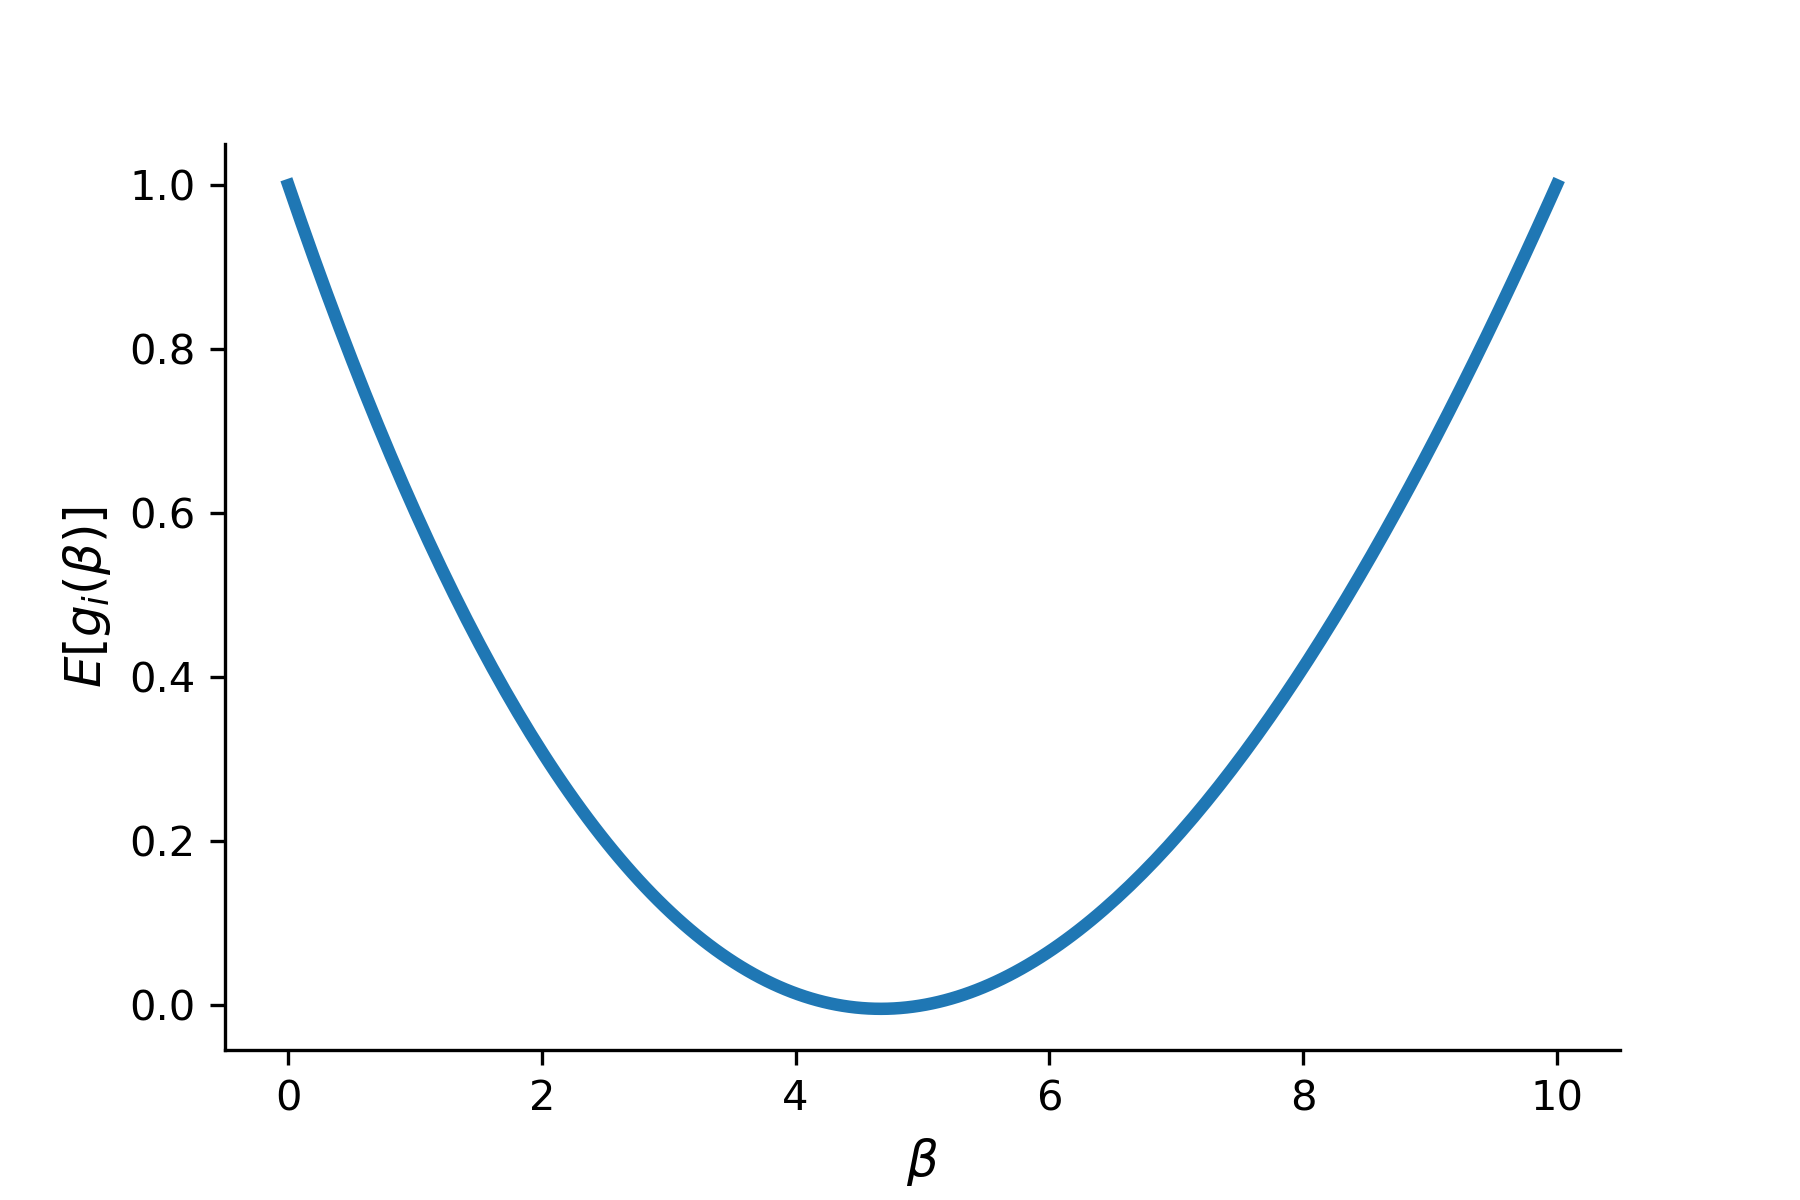
\includegraphics{material/fig-single-zero}}
\end{figure}
\end{frame}

%-------------------------------------------------------------------------------
%-------------------------------------------------------------------------------
\begin{frame}
\begin{figure}[htp]\centering
\scalebox{0.75}{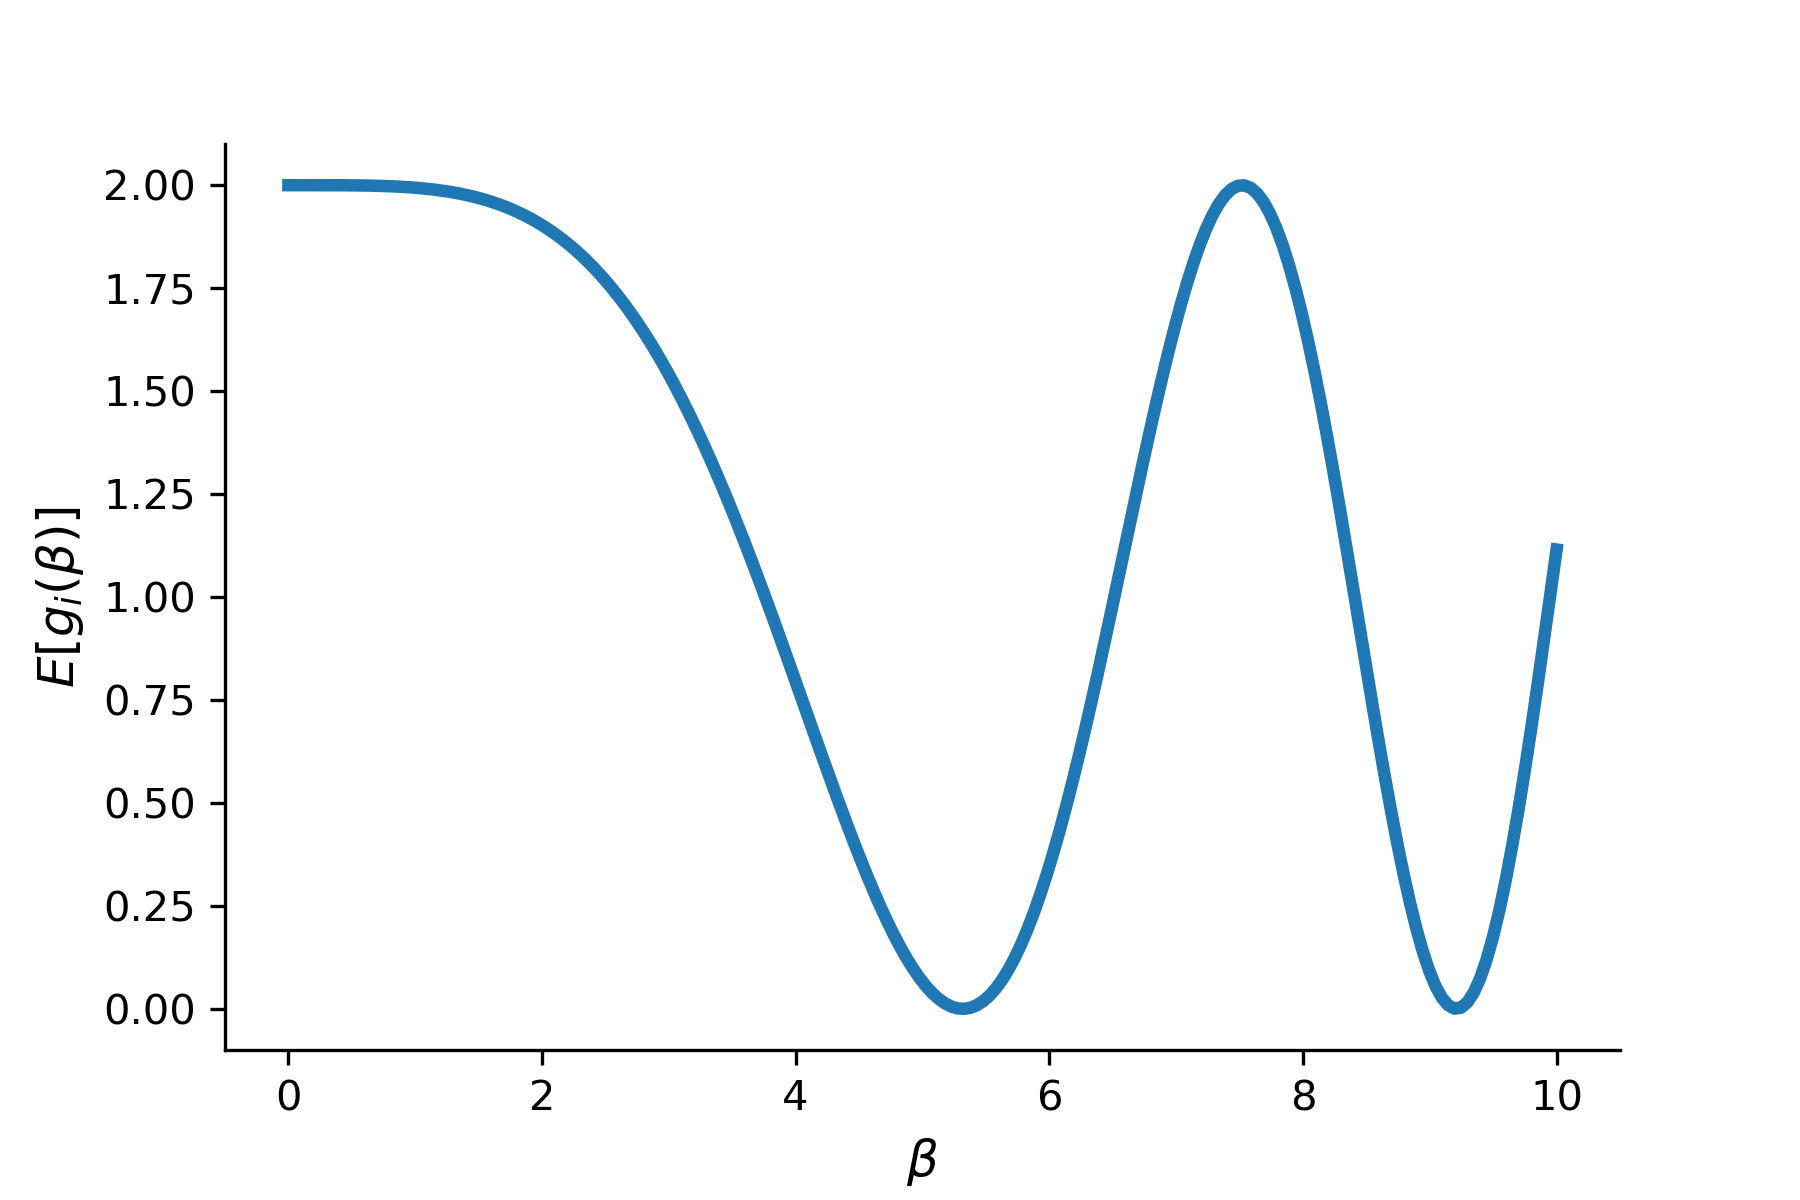
\includegraphics{material/fig-multiple-zero}}
\end{figure}
\end{frame}

%-------------------------------------------------------------------------------
%-------------------------------------------------------------------------------
\begin{frame}

\begin{itemize}
\item Necessary condition for identification is that $m \geq p$. When $m \leq p$, i.e. there are fewer equations to solve than parameters, there will
typically be multiple solutions to the moment conditions.
\end{itemize}

\end{frame}
%-------------------------------------------------------------------------------
%-------------------------------------------------------------------------------
\begin{frame}

\begin{itemize}\setlength\itemsep{1em}
\item Let $G = E[\partial g_i(\beta_0) / \partial \beta]$. Rank condition is $rank(G) = p$. Necessary and sufficient for identification when $g_i(\beta)$ is linear in $\beta$.
\item In the general nonlinear case it is difficult to specify conditions for uniqueness of the solution to $E[g_i(\beta)] = 0$.
\end{itemize}

\end{frame}
%-------------------------------------------------------------------------------
%-------------------------------------------------------------------------------
\begin{frame}

\begin{itemize}\setlength\itemsep{1em}
\item m = p, exact identification, $\hat{g}(\hat{\beta}) = 0$ asymptotically
\item m > p, overidentification, $\hat{g}(\hat{\beta}) > 0$ asymptotically\vspace{0.3cm}
\end{itemize}

In the case of overidentification, the choice of $A$ matters and affects the estimator's asymptotic distribution.

\end{frame}
%-------------------------------------------------------------------------------
%-------------------------------------------------------------------------------
